\chapter{Background}
\label{ch:background}

This work examines the relationship between system and application performance in the context of systems comprised of CPUs and Nvidia GPUs.
To that end, 
Section~\ref{sec:sys-abstraction}            describes the relationship between software abstractions and the underlying system hardware,
Section~\ref{sec:gpu-sys-arch}               discusses how Nvidia graphics processing units (GPUs) fit into the computing system architecture,
Section~\ref{sec:interconnects}              describes the PCIe and NVLink interconnect systems used to couple GPUs to each other and the rest of the system,
Section~\ref{sec:cuda}                       details communication-related components and APIs of CUDA, the Nvidia GPU programming system,
Sections~\ref{sec:numa} and~\ref{sec:openmp} describe the Linux non-uniform memory access (NUMA) and OpenMP multiprocessing systems,
Section~\ref{sec:profiling}                  describes the Linux and CUDA components used in the proposed application profiler,
and Section~\ref{sec:system-descriptions}    documents the heterogeneous systems used as case studies in this work.

\section{System Communication Abstraction}
\label{sec:sys-abstraction}

Application access to computing systems is made through a stack of abstractions.
This work considers applications that interface with the system through CUDA, the Linux NUMA abstraction, and OpenMP.
Those API calls are implemented in various libraries, such as \texttt{libcudart.so} on Linux systems.
In turn, those libraries make use of system calls provided by the operating system.
The operating system interfaces with various drivers, including the Nvidia GPU drivers and the interconnect drivers, to make use of the underlying hardware.
Figure~\ref{fig:app-abstraction} shows a schematic of this stack.

\begin{figure}[ht]
    \centering
    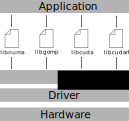
\includegraphics[width=0.5\textwidth]{figures/generated/app-abstraction.pdf}
    \caption[System abstraction]{
		The application interacts with the underlying hardware through libraries, the operating system, and drivers.
	}
    \label{fig:app-abstraction}
\end{figure}

Through these layers of abstraction, the underlying communication capabilities are modified.
For example, PCIe interconnects transfer data with packets, but the CUDA API does not expose the ability to create custom packets to send to the GPU.
Furthermore, the performance of the hardware is modified.
For example, when CUDA unified memory is used, some of the link bandwidth may be consumed by control signals that help ensure data coherence.
Chapters \ref{ch:explicit} and \ref{ch:unified} show how different uses of the CUDA API can achieve different performance on the same physical hardware.

\section{GPUs and System Architecture}
\label{sec:gpu-sys-arch}

Nvidia GPUs used in high-performance computing are fully-discrete accelerators.
From the software side, they demand explicit management through the Nvidia Compute Unified Device Architecture (CUDA) programming system: a set of C++ language extensions and libraries.
In a GPU-accelerated application, the CPU typically acts as a manager and ``offloads'' specialized compute tasks to the GPU.
From the hardware perspective, GPUs are separated from the CPU and memory by an interconnect link.
The GPU has its own local memory, which must be populated with data for the GPU to operate on.
For the rest of this thesis, we will refer to the system memory associated with that CPU as the ``CPU memory'' or ``system memory'', and the GPU's local memory as ``GPU memory''.
Finally, though not covered in this work, the GPU compute cores have dramatically different performance characteristics than CPU cores, and require specialized programming styles.

\begin{figure}[ht]
    \centering
    \begin{subfigure}[b]{0.2\textwidth}
        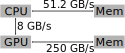
\includegraphics[width=\textwidth]{figures/generated/x86-kepler-bw.pdf}
        \caption{}
        \label{fig:x86-kepler-bw}
    \end{subfigure}
	~
	\begin{subfigure}[b]{0.2\textwidth}
        \includegraphics[width=\textwidth]{figures/generated/x86-pascal-bw.pdf}
        \caption{}
        \label{fig:x86-pascal-bw}
    \end{subfigure}
    ~
    \begin{subfigure}[b]{0.2\textwidth}
        \includegraphics[width=\textwidth]{figures/generated/p8-pascal-bw.pdf}
        \caption{}
        \label{fig:p8-pascal-bw}
    \end{subfigure}
    ~
    \begin{subfigure}[b]{0.2\textwidth}
        \includegraphics[width=\textwidth]{figures/generated/p9-volta-bw.pdf}
        \caption{}
        \label{fig:p9-volta-bw}
    \end{subfigure}
	\caption[Example system interconnect bandwidths]{
		Representative interconnect bandwidths between CPU and system memory, GPU and GPU memory, and CPU to GPU.
		(a) shows a c.2011 x86 system with an AMD Operton 6200 CPU~\cite{amd2012opteron6200} system, PCIe 2.0 x16, and Nvidia K20 GPU.
		(b) shows a c.2017 x86 system with an Intel Xeon Platinum 8180M~\cite{intel20188180m} CPU, PCIe 3.0 x16, and an Nvidia P100 GPU.
		(c) shows a c.2013 PowerPC system with an IBM Power8~\cite{stuechli2013power8} CPU, two-lane NVLink 1.0, and an Nvidia P100 GPU.
		(d) shows a c.2017 PowerPC system with an IBM Power9~\cite{thompto2016power9} CPU, three-lane NVLink 2.0, and an Nvidia V100 GPU.
	}
    \label{fig:gpu-sys-arch}
\end{figure}

Figure~\ref{fig:gpu-sys-arch} shows some example interconnect bandwidth numbers for some hypothetical systems.
In all cases, the bandwidth between the CPU or GPU and their respective memories is much higher than the bandwidth between the CPU and GPU.
In older systems and current x86 systems, that link may be an order of magnitude slower than the other interconnects.
The vastly different link performance makes data placement extremely important for application performance.

Figure~\ref{fig:x86-kepler-bw} is representative of a node of a supercomputer designed in 2012~\cite{ncsa2018bluewaters}.
Figure~\ref{fig:x86-pascal-bw} represents a similar system, with components updated to 2017.
Figure~\ref{fig:p8-pascal-bw} is a c.2013 system with an IBM Power8 CPU and NVLink 1.0.
Figure~\ref{fig:p9-volta-bw} represents next-generation interconnect bandwidths present in the Summit~\cite{ornl2018summit} and Sierra~\cite{llnl2018sierra} supercomputers delivered in 2018.

\section{PCIe and NVLink Interconnects}
\label{sec:interconnects}

Modern systems with discrete GPUs feature either NVLink or PCIe accelerator interconnects.
These interconnects couple the GPUs to the CPUs and/or other GPUs.
Table~\ref{tab:interconnect-overview} summarizes the theoretical bandwidth of common interconnect configurations.
Figure~\ref{fig:interconnect-cartoon} shows example PCIe and NVLink topologies.
Section~\ref{sec:cuda-peer} describes how these topologies affect parts of the CUDA peer-communication API.

\begin{table}[ht]
	\centering
	\caption[Interconnect performance summary]{
		Theoretical performance for common interconnect configurations.
		Only NVLink configurations used in the case studies are shown below.
		PCIe 3.0 x16 is included for reference, as most PCIe 3.0-attached GPUs use 16 lanes.
	}
	\label{tab:interconnect-overview}
	\begin{tabular}{cccc}
		\hline
		\textbf{Interconnect}      & \textbf{Bandwidth}   & \textbf{Year} & \textbf{Architecture} \\ \hline
		\textbf{PCIe 3.0}          & 15.8 GB/s (16 lanes) & 2012          & Tree                  \\ \hline
		\textbf{NVLink 1.0 / NVHS} &   20 GB/s (1 lanes)  & 2016          & Point-to-Point        \\ \hline
		\textbf{NVLink 1.0 / NVHS} &   40 GB/s (2 lanes)  & 2016          & Point-to-Point        \\ \hline
		\textbf{NVLink 2.0 / NVHS} &   75 GB/s (3 lanes)  & 2017          & Point-to-Point        \\ \hline
	\end{tabular}
\end{table}

\begin{figure}[ht]
    \centering
	\begin{subfigure}[b]{0.4\textwidth}
		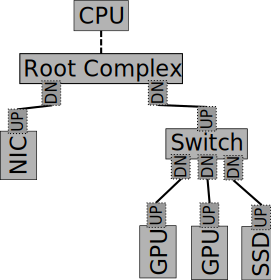
\includegraphics[width=\textwidth]{figures/generated/pcie-example.pdf}
		\caption[]{}
		\label{fig:pcie-cartoon}
    \end{subfigure}
    ~
    \begin{subfigure}[b]{0.4\textwidth}
		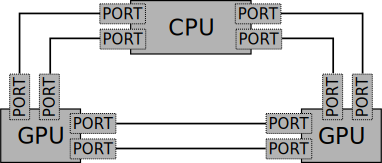
\includegraphics[width=\textwidth]{figures/generated/nvlink-example.pdf}
		\caption[]{}
		\label{fig:nvlink-cartoon}
    \end{subfigure}
    \caption[Example PCIe and NVLink interconnect topologies]{
		(a) An example PCIe topology, showing the root complex at the root of the tree, with endpoints and switches connected by links.
		(b) An example NVLink topology, with each device supporting four NVLinks, and using two to connect to each of its neighbor devices.
	}
    \label{fig:interconnect-cartoon}
\end{figure}

The Nvidia DGX-1 system (Section~\ref{sec:dgx1}) uses PCIe to connect CPUs to GPUs, and single-lane NVLink 1.0 to connect amongst GPUs.
The IBM S822LC system (Section~\ref{sec:s822lc}) uses two NVLink 1.0 lanes to connect pairs of devices, with each lane operating at 20 GB/s.
The IBM AC922 system (Section~\ref{sec:ac922}) uses three NVLink 2.0 lanes to connect pairs of devices, with each lane operating at 25 GB/s.

\subsection{PCIe}

Peripheral Component Interconnect Express (PCIe) is an expansion bus standard~\cite{pcie10}.
PCIe components form a tree, rooted at the \textit{root complex}.
PCIe devices such as GPUs or SSDs are \textit{endpoints}, with a single upstream port and no downstream ports.
Data is sent point-to-point between participating endpoints and/or the root complex via unique PCIe addresses.
The topology also may include \textit{switches}, components with a single upstream port and multiple downstream ports.
Switches do not receive data packets, and are only used to extend the topology.
Components are connected by PCIe \textit{links}, each of which consists of one to 32 lanes.
The total bandwidth of the link depends on the PCIe generation and the number of lanes.
Figure~\ref{fig:pcie-cartoon} shows an example topology.
The PCIe 3.0 specification~\cite{pcie30} was finalized in 2010, and the first Nvidia GPUs to support it were some Kepler-architecture products released in 2012~\cite{nyland2012inside}.

Table~\ref{tab:pcie-lane-rates} shows single-lane PCIe bandwidths from generation $1.0$ to $3.0$.
Physically, each PCIe lane has four wires, divided into two differential signaling pairs.
A PCIe 3.0 x16 interconnect therefore has 64 wires.
In PCIe 3.0, each signaling pair operates at 8 Gb/s.
With a 128b/130b encoding, this gives PCIe 3.0 x16 a 15.8 GB/s unidirectional bandwidth.

\begin{table}[ht]
	\centering
	\caption[PCIe lane transfer rates]{PCIe lane transfer rates}
	\label{tab:pcie-lane-rates}
	\begin{tabular}{cccc}
		\hline
		\textbf{PCIe Revision} & \textbf{Signaling Rate} & \textbf{Encoding} & \textbf{Line Bandwidth} \\ \hline
		\textbf{1.0}           & $2.5$ GT/s                & $8$b/$10$b            & $250$   MB/s      \\ \hline
		\textbf{2.0}           & $5.0$ GT/s                & $8$b/$10$b            & $500$   MB/s      \\ \hline
		\textbf{3.0}           & $8.0$ GT/s                & $128$b/$130$b         & $984.6$ MB/s      \\ \hline
	\end{tabular}
\end{table}

\subsection{NVLink}

NVLink is a communication protocol developed by Nvidia.
Current NVLink implementations use the proprietary high-speed signaling interconnect NVHS \cite{harris2016insidepascal}.
Like PCIe, each NVLink connects two devices.
Unlike PCIe, there is no concept of upstream or downstream ports, and devices may have multiple ports.
Multiple links may connect devices, in which case the links are combined to contribute to the available bandwidth between devices.
Figure~\ref{fig:nvlink-cartoon} shows an example topology.
The NVLink 1.0 systems in this work allow each device to have four NVLink lane connections, with each lane running at 20 GB/s~\cite{nvidia2017dgx1},~\cite{nvidia2016p100}.
The NVLink 2.0 systems in this work allow each device to have six NVLink lanes at 25 GB/s each~\cite{nvidia2017v100}.

Physically, each bidirectional lane has 32 wires, divided evenly into two unidirectional sublinks of eight differential pairs~\cite{harris2016insidepascal}.
Each pair operates at 20 Gb/s for NVLink 1.0 and 25 Gb/s for NVLink 2.0.
This means a 2-lane NVLink 1.0 has 64 wires.
The improved bandwidth of 2-lane NVLink 1.0 vs. PCIe 3.0 is directly attributable to the signaling rate on the wires.

\section{CUDA}
\label{sec:cuda}

Nvidia's CUDA (Compute Unified Device Architecture) is a programming system for enabling general-purpose computation on Nvidia GPUs (graphics processing units).
CUDA is a set of C extensions and libraries for interfacing with GPUs.
Nvidia provides a compiler, \texttt{nvcc}, for generating CUDA-enabled binaries.

CUDA provides a set of runtime and driver APIs for the developer to manage the allocation and movement of data between the host and device memory.
From its inception, CUDA provided comprehensive APIs for developers to mitigate application performance shortfalls stemming from the relatively limited performance of host-device communication links.
As the capabilities of GPUs and host systems have improved, CUDA has provided simpler, higher-level APIs that require less programmer effort.
This section describes CUDA memory-management capabilities and the historical context of their introduction.

The CUDA API has an associated version number that defines which CUDA actions are made available by that API.
CUDA-capable hardware advertises a specific compute capability (CC) that defines what CUDA actions are supported by that GPU.
Although the CUDA API may expose particular capability, the GPU may need a sufficiently high CC to take advantage of it.
This section references both these version systems when discussing CUDA features.

This work focuses on the performance of explicit CUDA memory management and the CUDA unified memory system.
There is a third set of transfer capabilities that fall under the umbrella of remote-mapping or ``zero-copy'' memory.
These techniques are subsumed by unified ,emory, though making use of them typically requires hints to the CUDA system.
Once the flexibility of the unified memory system improves, it will be important to revisit the performance implications of zero-copy memory.

\subsection{Basic CUDA Memory and System Memory}
\label{sec:basic-cuda}

Prior to the introduction of unified virtual addressing (see Section~\ref{sec:uva}), the CUDA memory space was composed of multiple address spaces: one for the host, and one for each GPU~\cite{schroeder2011peer}.
Data was explicitly allocated in those address spaces through \texttt{cudaMalloc}.
Standard C/C++ memory allocation techniques (\texttt{malloc}/\texttt{new}, \texttt{free}/\texttt{new}) are used for managing memory on the host.
\texttt{cudaMemcpy} is used to move data between address spaces, whether the host and device or between devices.
Since each device has a separate address space, the programmer explicitly instructs \texttt{cudaMemcpy} how to move data with \texttt{cudaMemcpyHostToDevice}, \texttt{cudaMemcpyDeviceToHost}, or \texttt{cudaMemcpyDeviceToDevice}.
Basic CUDA memory management runtime calls are described in Table~\ref{tab:cuda-basic-apis}.

\begin{table}[ht]
	\centering
	\caption[Basic memory-management APIs]{
		Basic CUDA and C/C++ memory-management APIs.
	}
	\label{tab:cuda-basic-apis}
	\begin{tabular}{cc}
		\hline
		\textbf{CUDA API}          & \textbf{Description}                         \\ \hline
		\texttt{cudaSetDevice()}   & Associate a device with the host thread.     \\ \hline
		\texttt{cudaMalloc()}      & Allocate memory on the device.               \\ \hline
		\texttt{cudaFree()}        & Free memory on the device.                   \\ \hline
		\texttt{cudaMemcpy()}      & Copy data between to,from,and between GPUs.  \\ \hline
		\texttt{cudaMemcpyPeer()}  & Copy data between GPUs without CPU involved. \\ \hline
		\hline 
		\textbf{C/C++ API}         & \textbf{Description}                         \\ \hline
		\texttt{new / malloc()}    & Allocate pageable memory on the system heap. \\ \hline
	\end{tabular}
\end{table}

\texttt{CudaMemcpy} is only partially asynchronous with respect to the host (\cite{nvidia2014cuda60runtime}, ch. 1).
It will return once the pageable source allocation is safe to modify, but possibly before the data has finished moving to the device.
This impacts the design of the performance characterization routines in Chapter~\ref{ch:explicit}.
\texttt{CudaMemcpyPeer} initiates a DMA copy from one GPU to another, without involving the host.
This can improve the bandwidth of the transfer between supported devices.
The impact of this peer access is also described in Chapters~\ref{ch:explicit} and~\ref{ch:unified}.

This API definition imposes the following basic structure on all CUDA programs, which remains essentially unchanged through CUDA 9.1.
\begin{enumerate}
	\item Allocate memory on the host with \texttt{new}/\texttt{malloc}.
	\item Initialize memory on the host.
	\item Allocate memory on the device with \texttt{cudaMalloc}.
	\item Copy initialized data from the host to the device with 
	\newline \texttt{cudaMemcpy(..., cudaMemcpyHostToDevice)}.
	\item Launch CUDA kernels.
	\item Copy results back to the host with \texttt{cudaMemcpy(...,} 
	\newline \texttt{cudaMemcpyDeviceToHost)}.
	\item Free CUDA allocations with \texttt{cudaFree}.
\end{enumerate}

Unified virtual addressing (Section~\ref{sec:uva}) and unified memory (Section ~\ref{sec:unified-cc3}) allow the data transfer steps to happen implicitly on supported systems.

\subsection{Page-Locked Memory}
\label{sec:pinned-memory}

The GPU uses direct memory access (DMA) to copy data to and from the host.
When \texttt{cudaMemcpy} is invoked, the CPU instructs the GPU to copy a region of host memory to the device memory (or vise-versa), without the CPU being involved.
The host must guarantee that the memory to be accessed by the GPU will not be paged-out during the copy.
First, \texttt{cudaMemcpy} copies the data from the application address space to a piece of page-locked memory in the system memory managed by the CUDA driver, and then \texttt{cudaMemcpy} instructs the GPU to initiate the DMA from that page-locked region to the GPU memory.

The CUDA runtime functions in Table~\ref{tab:cuda-pinned-apis} are the core functions CUDA provides to make page-locked memory regions directly visible to the application.
When the application uses these APIs, the first copy from pageable host memory to page-locked host memory can be elided.
Section~\ref{sec:explicit-pageable-pinned-wc} demonstrates the performance improvement from skipping this first copy.
Overuse of page-locked memory on the host will degrade overall application performance or even impact system stability if the host system is not able to page as needed.

\begin{table}[ht]
	\centering
	\caption[CUDA pinned memory-management APIs]{
		CUDA pinned memory-management APIs.
	}
	\label{tab:cuda-pinned-apis}
	\begin{tabularx}{\textwidth}{M{1.5in} Y M{0.9in}}
		\hline
		\textbf{API}                & \textbf{Description}                    & \textbf{CUDA Version Introduced} \\ \hline
		\texttt{cudaMallocHost()}   & allocate page-locked memory on the host & 1.0~\cite{nvidia2007cuda10} \\ \hline
		\texttt{cudaFreeHost()}     & free page-locked memory on the host     & 1.0~\cite{nvidia2007cuda10} \\ \hline
		\texttt{cudaHostAlloc()}    & cudaMallocHost with additional options  & 3.0~\cite{nvidia2010cuda30} \\ \hline
		\texttt{cudaHostRegister()} & Page-lock a range of host memory        & 4.0~\cite{nvidia2011cudac40} \\ \hline
	\end{tabularx}
\end{table}

\begin{sloppypar}
\texttt{CudaHostAlloc} allows even more options, including the \texttt{cudaHostAllocPortable} and \texttt{cudaHostAllocWriteCombined} flags.
%3.2.4.2
\texttt{CudaHostAllocWriteCombined} causes a pinned allocation to be write-combined.
Writes to write-combined memory may be delayed and combined in a buffer to reduce the number of memory accesses.
Additionally, the host may not cache this data in L1 or L2 cache, freeing up those resources for other applications.
This may prevent unnecessary cache invalidations from occurring during the DMA.
Furthermore, coherency is not enforced, so data is not snooped on the PCIe bus, which can increase bandwidth by up to 40\% (\cite{nvidia2010cuda30}, 3.2.5.2).
Due to the possible lack of caching, this type of allocation makes sense for data that is not frequently read by the CPU, for example, data written once by the CPU before being sent to a GPU.
\end{sloppypar}

\texttt{CudaHostAllocPortable} allows all CUDA contexts to treat the memory as pinned, not just the context that performed the allocation.
This became the default with the introduction of unified virtual addressing.

\subsection{Unified Virtual Addressing}
\label{sec:uva}

Unified virtual addressing was introduced with compute capability 2.0 GPUs and CUDA 4.0 on 64-bit systems.
The host memory and the memory of each GPU are mapped into disjoint subsections of a single unified address space.

This enhancement simplifies several of the already-introduced CUDA memory management commands~(\cite{nvidia2011cudac40}, 3.2.7).
The \texttt{cudaMemcpyDefault} flag for \texttt{cudaMemcpy} instructs the CUDA system to automatically determine how to move data.
By examining the address of the pointers passed to \texttt{cudaMemcpy}, CUDA determines where which device the memory resides on and moves it accordingly.
This simplifies the programmer's use of \texttt{cudaMemcpy}, as \texttt{cudaMemcpyDefault} may be used everywhere.
There is also no need to call \texttt{cudaHostGetDevicePointer} for mapped allocations.
Furthermore, all mapped allocations are automatically accessible by all GPUs in the system, not restricted to the GPU that was active at the time of the allocation.
\texttt{CudaMemcpyPeer} is no longer needed for device-to-device memory copies; \texttt{cudaMemcpy} may be used instead.

\subsection{Peer Access and UVA}
\label{sec:cuda-peer}



Peer access was introduced with CUDA 4.0.
\texttt{CudaDeviceEnablePeerAccess()} allows CC 2.0+ devices to address memory in another device's address space~(\cite{nvidia2011cudac40}, 3.2.6.4).
For example, if GPU1 loads through a pointer to data on GPU0, the data will be directly fetched from GPU0 memory, at the cost of one PCIe transaction and one global memory load~\cite{schroeder2011peer}, and be cached in the L2 of GPU0.
Direct peer access requires compute capability 2.0, CUDA 4.0, Fermi+, and 64-bit system.
The availability of peer access may rely on a combination of interconnect topology and system hardware, summarized in Table~\ref{tab:cuda-peer-topology}.
When peer access is disabled, data transfers first pass through the host instead of allowing direct DMA between devices.

\begin{table}[ht]
	\centering
	\caption[System support for GPU-GPU peer access]{
		GPU-to-GPU connection, and whether peer access is supported for the systems considered in this work.
	}
	\label{tab:cuda-peer-topology}
	\begin{tabular}{ccc}
		\hline
		\textbf{Between GPUs with...}  & \textbf{System} &  \textbf{Peer Access} \\ \hline
		...a shared PCIe switch        & DGX-1           &  \checkmark           \\ \hline
		...different PCIe switches     & DXG-1           &  $\times$             \\ \hline
		...a direct NVLink connection  & S822LC          &  \checkmark           \\ \hline
		...no direct NVLink connection & S822LC          &  $\times$             \\ \hline
		...a direct NVLink connection  & AC922           &  \checkmark           \\ \hline
		...no direct NVLink connection & AC922           &  \checkmark           \\ \hline

	\end{tabular}
\end{table}

\subsection{Unified Memory with CC 3.0+ (Kepler+)}
\label{sec:unified-cc3}

The CUDA unified memory system was introduced with CUDA 6.0 and requires a GPU with SM architecture of 3.0 or higher~\cite{nvidia2014cuda60}.
CUDA unified memory~\cite{harris2013cudaunifiedmemory} provides a single pool of memory that is accessible from the CPU and GPU by a single pointer.
CUDA automatically migrates data between the physically distinct CPU and GPU memory as needed, allowing GPU kernels to access the memory as if it were in the global memory, and CPU functions to access the memory as if it were in the system memory.
Like mapped memory, this simplifies programming by removing the need for separate host and device allocations and explicit data transfers.
A summary of unified memory APIs is shown in Table~\ref{tab:cuda-um-apis}.

\begin{table}[ht]
	\centering
	\caption[CUDA unified memory-management APIs]{
		CUDA unified memory-management APIs.
		Initial CUDA 6.0 APIs and additional CUDA 8.0 APIs are shown.
	}
	\label{tab:cuda-um-apis}
	\begin{tabularx}{\textwidth}{cY}
		\hline
		\textbf{CUDA 6 and CC3.0+}           & \textbf{Description}                        \\ \hline
		\texttt{\_\_managed\_\_}             & Defines a global variable in managed memory \\ \hline
		\texttt{cudaMallocManaged()}         & allocate a unified memory region.           \\ \hline
		\texttt{cudaStreamAttachMemAsync()}  & Attach a managed allocation to a stream, instead of globally. \\ \hline \hline
		\textbf{CUDA 8 and CC6.0+}           & \textbf{Description}               \\ \hline
		\texttt{cudaMemPrefetchAsync()}      & Hint to prefetch memory to device  \\ \hline
		\texttt{cudaMemAdvise()}             & Hint about how memory will be used \\ \hline

	\end{tabularx}
\end{table}

The underlying data is only present in one location on the system, and in principle, unified memory allocations are automatically migrated towards their most recent use.
When a kernel is launched, all pages attached to that kernel's stream are bulk migrated to the destination GPU.
When the host program touches a page, that page is migrated back to the system memory.
In multi-GPU systems, data does not migrate between GPUs - all other GPUs receive peer mappings to the data, which is accessed over the PCIe bus (\cite{nvidia2014cuda60}, J.1.3).

Unified memory maintains coherence (i.e., all GPUs and the CPU have the same view of unified memory values) by disallowing concurrent accesses to managed data, including concurrent access to distinct managed allocations (\cite{nvidia2014cuda60}, J.2.2.1).
The CPU may access managed allocations after GPU execution has completed, where ``GPU execution'' refers to activity in a particular stream for stream-attached memory, or whole-GPU otherwise.
For stream-attached memory, completion of GPU execution can be guaranteed by any stream-synchronizing call.
For whole-GPU memory, completion is guaranteed by stream synchronization when only one stream is executing on the GPU,\footnote{e.g., \texttt{cudaStreamSynchronize()}} or by any call that is fully synchronous with respect to the host.\footnote{e.g., \texttt{cudaDeviceSynchronize()}}
The GPU is considered to be active even if it is not accessing managed data.
Concurrent inter-GPU accesses are allowed, as are concurrently-executing kernels on a single GPU (\cite{nvidia2014cuda60}, J.2.2.2).

\subsection{Unified Memory with CC 6.0+ (Pascal+)}
\label{sec:unified-cc6}

With CUDA 8 and for GPUs with CC 6.0+, GPU page faulting provides a more fine-grained data transfer mechanism~\cite{nvidia2017cuda80}.
Instead of moving all managed allocations to the GPU prior to a kernel launch, the GPU will fault if it accesses a page that is not in its memory.
The page is either migrated to the GPU to serve that access, or the page is mapped into the GPU address space to be accessed over the host-device interconnect.
Unlike unified memory with CC 3.0, pages can migrate between GPUs on peer accesses (\cite{nvidia2017cuda80}, J.1.4).
The GPU page faulting mechanism lifts all restrictions on simultaneous access to data (\cite{nvidia2017cuda80}, J.2.2.1).
However, intensive interleaving of CPU and GPU accesses to a page can cause excessive migrations and result in severe performance degradation.

CC 6.0+ also brings 49-bit virtual addressing to cover the 48-bit virtual addressing of modern CPUs and the GPU memory.
This allows CUDA to support managed allocations larger than the GPU memory.
The total amount of managed allocations still cannot be larger than the system memory (\cite{nvidia2017cuda80}, J.1.3).

\texttt{CudaMemPrefetchAsync()} hints to the unified memory system that a particular device will soon be accessing a unified memory allocation.
This may cause the system to migrate the specific region of memory over to the referenced device.
This hint is used in Chapter~\ref{ch:explicit} in some of the unified memory characterizations.

\texttt{CudaMemAdvise()} hints to the unified memory system how a particular region of memory can be used.
\texttt{CudaMemAdviseSetReadMostly} causes the hinted device to establish a read-only copy of a page, instead of taking complete ownership of a page on access.
Any writes to that page become expensive, as all read-only copies must be invalidated.
This cost is not evaluated in this work.
\texttt{CudaMemAdviseSetPreferredLocation} hints to the driver that data migration of the page away from the device should be avoided.
This may cause the system to establish a remote mapping for the data, instead of migrating the page.
\texttt{CudaMemAdviseSetAccessedBy} hints to the driver that the device will access the memory region.
It causes the page to be mapped in the device page table for as long as possible, to prevent page faults on access.

\subsection {Unified Memory with CC 7.0+ (Volta+) }
Though not examined in this work, Volta GPUs contain the necessary hardware for more intelligent migration of pages.
When support is added in the Nvidia driver, access counters will be used to trigger page migrations of hot pages, instead of on each access.
The system will also detect thrashing, and temporarily prevent page faults to allow faster progress on each device.
On POWER9 systems, the CPU and GPU have access to each other's page translation hardware, allowing memory accesses on the CPU to be served from the GPU and cached on the CPU.
Furthermore, the CPU can execute atomic operations on locations in GPU memory without a page migration~\cite{sakharnykh2017unified}.

\section{Linux Non-Uniform Memory Access}
\label{sec:numa}

Linux includes a system for exposing non-uniform memory access architectures (NUMA) to applications.
In NUMA systems, memory is divided into multiple \textit{nodes}~\cite{numa2012}.
Processors and devices have the same access characteristics when accessing memory in a particular node.
Nodes have \textit{affinity} to processors and devices, indicating the processors and devices which can access that node with the best performance.

This is particularly relevant on multi-socket systems, though some single-socket systems also feature NUMA characteristics.
For example, every system considered by this work and described in Section~\ref{sec:system-descriptions} is a NUMA system.
On the AC922 (Figure~\ref{fig:topo-ac922-simple}), GPU0 is directly connected to CPU0 and GPU2 is directly connected to CPU1.
If an allocation on CPU0 were to be copied to GPU2, the data would traverse the CPU-CPU X bus, and then the CPU-to-GPU NVLink.
On the other hand, if an allocation on CPU1 were to be copied to GPU2, that data would only have to traverse the NVLink.
This can have a substantial effect on available bandwidth, as shown in Figure~\ref{fig:numa-bw-example}.
Chapters~\ref{ch:explicit} and ~\ref{ch:unified} show these effects in more detail.

\begin{figure}[H]
    \centering
	\includegraphics[width=0.5\textwidth]{figures/generated/ac922_numa-bw.pdf}
    \caption[Example of NUMA bandwidth effects on AC922]{Example of NUMA bandwidth effects on AC922}
    \label{fig:numa-bw-example}
\end{figure}

Applications can leverage the numactl~\cite{wickman2015numactl} library to affect their own NUMA execution policy.
This policy controls on which CPUs processes may execute, and on which NUMA nodes memory is allocated.
Numactl is used in this work to ensure that data is allocated and programs execute on specific CPUs as needed to exercise different underlying hardware links.
Listing~\ref{lst:numa-bind-node} shows a C++ function that takes the operating system NUMA node ID as an integer argument and binds the executing thread and its allocations to that node.
Lines 6 and 7 allocate a \texttt{bitmask}, and set the bit corresponding to the NUMA node.
\texttt{Numa\_bind()} in line 8 forces execution and allocations to occur on the nodes in the nodemask.

\begin{minipage}{\linewidth}
\begin{lstlisting}[language=C++, caption=Binding to NUMA nodes., label=lst:numa-bind-node, numbers=left]
static inline void 
numa_bind_node(const int node) {
  if (-1 == node) {
	numa_bind(numa_all_nodes_ptr);
  } else if (node >= 0) {
	struct bitmask *nodemask = numa_allocate_nodemask();
	nodemask = numa_bitmask_setbit(nodemask, node);
	numa_bind(nodemask);
	numa_free_nodemask(nodemask);
  } else {
	exit(1);
  }
}
\end{lstlisting}
\end{minipage}

The benchmarks in this paper also initialize numactl with calls to \texttt{numa\_set\_strict(1)} and \texttt{ numa\_set\_bind\_policy(1)}, which ensure that NUMA will cause the program to exit on an error, and that if the memory cannot be allocated on the requested NUMA node, the allocation will fail instead of falling back to a different node.

\section{OpenMP}
\label{sec:openmp}

OpenMP is a shared-memory processing system that uses compiler directives and library functions to allow applications to implement shared-memory parallel processing techniques~\cite{openmp2013}.
Among other more sophisticated approaches, OpenMP allows hint-assisted parallelization of nested loops through compiler directives.
This work uses OpenMP to use multiple CPU threads while transferring data between the CPU and the GPU during the unified memory characterization in Chapter~\ref{ch:unified}. 
Multiple CPU threads are used to ensure that the CPU is generating sufficient memory traffic to saturate its memory controllers and make the maximal demands of the unified memory system.
There is a runtime overhead of entering the parallelized region, which affects the design of the benchmarks.

Many microbenchmarks in this work rely on execution of threads on particular NUMA nodes.
The \texttt{numa\_bind($node$)} function binds the current process and all child processes to the provided node, but OpenMP does not necessarily implement worker threads as children of the current thread.
Algorithm~\ref{alg:omp-numa-bind} is used to bind all OpenMP threads to a NUMA node.
A full OpenMP thread team is created, and each of those threads individually binds itself to the provided NUMA node.

\begin{algorithm}
	\caption[Bind OpenMP threads to a NUMA node]{
		Algorithm to bind all OpenMP threads to a NUMA node.
	}
	\label{alg:omp-numa-bind}
	\begin{algorithmic}[1]
		\Statex
        \Function{omp\_numa\_bind\_node}{$dev$}
        \State \texttt{bind\_cpu($dev$)}
        \For{all worker threads}
        \State \texttt{bind\_cpu($dev$)}
        \EndFor
        \EndFunction
		
	\end{algorithmic}
\end{algorithm}

\section{Profiling Tooling}
\label{sec:profiling}

\subsection{CUDA Events}

An event is a special kind of operation that is performed in a CUDA stream.
CUDA events allow the CUDA runtime to set and query noteworthy milestones in the sequence of stream operations without stalling the stream.
These events may be used as a lightweight method for measuring how much time CUDA operations take without also measuring the time taken to synchronize the stream.
Events are created with \texttt{cudaEventCreate()}, destroyed with \texttt{cudaEventDestroy()}, and inserted into a stream with \texttt{cudaEventRecord()}.
\texttt{CudaEventSynchronize()} blocks the calling thread until a particular event has been completed in the stream.
\texttt{CudaEventElapsedTime()} returns the number of milliseconds that have elapsed between two completed events.
Listing~\ref{lst:cuda-events} shows an example of measuring time of hypothetical CUDA operation \texttt{cudaSomeAsyncOperation()} taking place in the \texttt{stream} stream.

\begin{minipage}{\linewidth}
\begin{lstlisting}[language=C++, caption=Measuring time with CUDA events., label=lst:cuda-events, numbers=left]
// Declare variables
float millis;
cudaEvent_t start, stop;
cudaStream_t stream;

// Create events
cudaEventCreate(start);
cudaEventCreate(stop);

// Insert events into stream
cudaEventRecord(start, stream);
cudaSomeAsyncOperation(..., stream);
cudaEventRecord(stop, stream);

// Wait for events to finish before computing time
cudaEventSynchronize(stop);
cudaEventElapsedTime(&millis, start, stop);
\end{lstlisting}
\end{minipage}

Lines $7$ and $8$ create the events that will wrap the operation to be timed.
Lines $11$ and $13$ insert the \texttt{start} and \texttt{stop} events around the operation to be timed.
Line $16$ blocks until the events have finished, then line $17$ produces the milliseconds elapsed between the \texttt{start} and \texttt{stop} events.

\subsection{CUDA Profiling Tools Interface}
\label{sec:cupti}

The CUDA Profiling Tools Interface~\cite{nvidia2017cupti} (CUPTI) ``provides...detailed information about how applications are using the GPU in a system.''
Users may inject code into the entry and exit point of every CUDA C runtime and CUDA driver API function call.
Additionally, users may configure and query hardware and software event counters to get insight into the operation of the GPU and CUDA stack.
The event counters include instruction count, instruction throughput, memory loads/stores, memory throughput, cache hits/misses, branches and custom profile triggers.
Chapter~\ref{ch:future} describes how CUPTI can be used to record memory allocations, kernel arguments, and timestamps to build a model of the application execution.

\subsection{\texttt{LD\_PRELOAD}}
\label{sec:ldpreload}

LD\_PRELOAD~\cite{kerrisk2017ld} is a mechanism by which the ld linker will load additional user-specific shared objects before any others.
If a function definition is present in a pre-loaded shared object, it will override the implementation present in later objects.
When combined with \texttt{dlsym()}~\cite{kerrisk2017dlysm}, it can be used to inject code into the entry of library calls in dynamically-linked binaries.
Chapter~\ref{ch:future} describes how LD\_PRELOAD can be used to infer information about application activity based on generic library calls.


\section{Benchmark Library}
\label{sec:benchmark}

This work makes use of the Google Benchmark library~\cite{google2018benchmark} as a harness for the developed custom microbenchmarks.
Benchmark automatically determines the number of iterations to run based on the number of inputs and the desired CPU time.
Benchmark allows repeated runs, and can report individual and aggregated statistics.
This work makes uses of repeated runs, and presents results in terms of mean values and standard deviations.
Benchmark also supports manual or automatic timing.
An example of the basic layout of an automatic timing benchmark is shown in Listing~\ref{lst:benchmark-automatic}.
Microbenchmarks using Benchmark are written in C++, and have a setup phase, an interaction phase, and a teardown phase.

\begin{minipage}{\linewidth}
\begin{lstlisting}[language=C++, caption=Benchmark with automatic timing., label=lst:benchmark-automatic, numbers=left]
#include <benchmark/benchmark.h>
static void BM_Foo(benchmark::State& state) {
  for (auto _ : state) {
	  state.PauseTiming();
	  // Time elapsed here will not be counted
	  state.ResumeTiming();
	  foo();
	}
}
BENCHMARK(BM_Foo);
\end{lstlisting}
\end{minipage}

Lines $2$-$9$ define a Benchmark function, which is registered to be run in line $10$.
The loop body in lines $4$ through $7$ is executed and timed automatically by the framework, and the average time is recorded.
Any part of the loop body that should not be timed can be wrapped in \texttt{state.PauseTiming()} and \texttt{state.ResumeTiming()}.
This allows for per-iteration setup code to not be timed.
The number of loop iterations is automatically controlled by the benchmark suite based on the number of arguments and desired run time.
For the benchmarks presented in this work, there are tens of thousands of iterations for small transfers, and as few as a single transfer test for large iterations.
The mean time is reported as a result of the benchmark.
This process is then repeated multiple times to determine a standard deviation of the measurement.

Some of the microbenchmarks in this work make use of CUDA events to accurately measure the time taken by various CUDA operations.
Benchmark supports this by allowing each microbenchmark to record and report its own iteration time.
For example, consider Listing~\ref{lst:benchmark-manual}.

Benchmark provides a \texttt{DoNotOptimize(<expr>)} function, which forces the result of \texttt{<expr>} to be placed in a register.
It does not prevent any optimization of \texttt{<expr>}, including replacing it with a statically-known value.
Benchmark also provides a \texttt{ClobberMemory()} function, which forces all pending global memory writes to be completed.
Through these two functions, the microbenchmarks can ensure that specific memory operations are completed and not optimized away.

\begin{minipage}{\linewidth}
\begin{lstlisting}[language=C++, caption=Benchmark with manual timing., label=lst:benchmark-manual, numbers=left]
#include <benchmark/benchmark.h>
static void BM_Foo(benchmark::State& state) {
  cudaEvent_t start, stop;
  cudaEventCreate(start);
  cudaEventCreate(stop);
  float msec;

  for (auto _ : state) {
    cudaEventRecord(start, NULL);
    ... // cuda operation to benchmark
    cudaEventRecord(stop, NULL);
    cudaEventSynchronize(stop);
    cudaEventElapsedTime(&msec, start, stop);
    state.SetIterationTime(msec / 1000);
  }
}
BENCHMARK(BM_Foo)->UseManualTime();
\end{lstlisting}
\end{minipage}

Now, when the benchmark is registered in line 17, the framework is informed that the benchmark loop iteration will report its own time.
Instead of the framework timing the loop body in lines 9-14, CUDA events are used to measure the operation time.
The iteration time is manually set in line 14.

Although Benchmark also supports multithreaded benchmarking, the microbenchmarks developed for this work do not use it.
Benchmark does not directly support thread synchronization within each benchmark iteration, which is needed to accurately measure the performance of using multiple threads to move memory.

\section{System Descriptions}
\label{sec:system-descriptions}

Three high-performance heterogeneous systems are used in this work: an IBM S822LC for High Performance Computing~\cite{caldeira2016s822lc}, an IBM AC922~\cite{caldeira2018ac922}, and an Nvidia DGX-1~\cite{nvidia2017dgx1}.
All systems feature multiple GPUs and multiple socketed CPUs.
Their key differences are in CPU architecture (64-bit little-endian PowerPC for S822LC and AC922, x86-64 for DGX-1), number of GPUs (4 for the IBM machines, 8 for Nvidia), and GPU connection topology (NVLink 1.0 for S822LC, NVLink 2.0 for AC922, and hybrid PCIe 3.0 / NVLink 1.0 for DGX-1).

\subsection{Nvidia DGX-1}
\label{sec:dgx1}

\begin{table}[ht]
    \centering
    \caption[Nvidia DGX-1 architecture summary]{
		Nvidia DGX-1 architecture summary.
	}
    \label{tab:dgx1}
    \begin{tabular}{cc}
    \hline
    \textbf{Component}            & \textbf{Specification}                                      \\ \hline
    \textbf{CPU}                  & \makecell{2x Intel Xeon E5-2698 v4 \\ 40C / 80T \\ 2.2 GHz} \\ \hline
    \textbf{System Memory}        & 512 GB DDR4                                                 \\ \hline
	\textbf{GPU}                  & 4 Nvidia P100                                               \\ \hline
	\textbf{CPU/GPU Interconnect} & NVLink 1.0 (1 lane) / PCIe 3.0                              \\ \hline
	\textbf{CUDA}                 & 8.0, driver 384.125                                         \\ \hline
	\textbf{Kernel}               & 4.4.0-79                                                    \\ \hline
    \end{tabular}
\end{table}

\begin{figure}[ht]
    \centering
	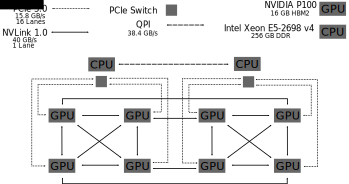
\includegraphics[width=0.8\textwidth]{figures/generated/dgx1-hardware.pdf}
    \caption[Nvidia DGX-1 architecture schematic]{
		Nvidia DGX-1 architecture schematic.
		Interconnect legends are subtitled with theoretical maximum transfer rates.
		Each of the four NVLink lanes on a GPU is used to connect it to one other GPU.
		CPUs are connected to GPUs by PCIe 3.0 x16 interconnects.
	}
    \label{fig:topo-dgx-simple}
\end{figure}

Table~\ref{tab:dgx1} and Figure \ref{fig:topo-dgx-simple} summarize the Nvidia DGX-1 system architecture.
The Nvidia DGX-1 machine consists of two symmetric sections \cite{nvidia2017dgx1}.
Each section consists of one 20-core Intel Xeon E5-2698v4 CPUs with 2-way SMT.
Each CPU is connected to 256GB of DDR4 RAM, and each section makes up a Linux NUMA node.
Each section has 4 Nvidia Tesla P100 GPUs coupled by single NVLinks.
The sections are connected by an Intel 9.6GT/s QPI bus between the CPUs providing 38.4 GB/s of bidirectional bandwidth, as well as NVLinks between corresponding GPUs.
The first CPU socket hosts the majority of the PCI devices on the system, including the network interfaces and the disks.
The CPU/GPU device affinity is relatively simple: CPU0 is directly connected to GPUs 0-3 and CPU1 is directly connected to GPUs 4-7.
Every GPU is directly connected to all local GPUs in its cluster, as well as one outside.

\subsection{IBM S822LC for High Performance Computing}
\label{sec:s822lc}

\begin{table}[ht]
    \centering
    \caption[IBM S822LC architecture summary]{IBM S822LC architecture summary.}
    \label{tab:minsky}
    \begin{tabular}{cc}
    \hline
    \textbf{}                     & \textbf{Specification}                         \\ \hline
    \textbf{CPU}                  & \makecell{2x IBM Power8 \\ 20C / 80T \\ 4 GHz} \\ \hline
    \textbf{System Memory}        & 512 GB DDR4                                    \\ \hline
	\textbf{GPU}                  & 4 Nvidia P100                                  \\ \hline
	\textbf{CPU/GPU Interconnect} & NVLink 1.0 (2 lanes)                           \\ \hline
	\textbf{CUDA}                 & 9.1.85, driver 390.31                          \\ \hline
	\textbf{Kernel}               & 4.4.0-96                                       \\ \hline
    \end{tabular}
\end{table}

\begin{figure}[ht]
	\caption[IBM S822LC architecture schematic]{
		IBM S822LC architecture schematic.
		Interconnect legends are subtitled with theoretical maximum transfer rates.
		The four NVLink lanes on a GPU are bonded into two two-lane pairs to connect it to the neighboring CPU and GPU.
	}
    \centering
	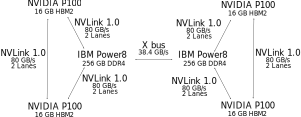
\includegraphics[width=0.8\textwidth]{figures/generated/minsky-hardware.pdf}
    \label{fig:topo-minsky-simple}
\end{figure}

Table~\ref{tab:minsky} and Figure~\ref{fig:topo-minsky-simple} summarize the hardware configuration.
The IBM S822LC machine features two POWER8 CPUs and four Nvidia P100 GPUs~\cite{caldeira2016s822lc}.
Each POWER8 CPU has 10 cores, with 8-way simultaneous multithreading, and is attached to 256GB of DDR4 memory for a total of 160 threads and 512 GB of memory.
Each POWER8 CPU and associated memory make up a Linux NUMA node.
Each POWER8 CPU is part of a fully-connected triad of one POWER8 CPU and two P100 GPUs.
Each device in the triad is connected by a gang of two NVLink 1.0 lanes for a total bidirectional bandwidth of 80 GB/s.
The two triads are connected at the POWER8 CPUs by an IBM SMP X bus with 38.4 GB/s of bidirectional bandwidth.

\subsection{IBM AC922}
\label{sec:ac922}

\begin{table}[ht]
	\caption[IBM AC922 architecture summary]{IBM AC922 architecture summary}
    \centering
    \label{tab:ac922}
    \begin{tabular}{cc}
    \hline
    \textbf{}                      & \textbf{Specification}                           \\ \hline
    \textbf{CPU}                   & \makecell{2x IBM Power9 \\ 40C 160T \\ 3.0 GHz } \\ \hline
    \textbf{System Memory}         & 1TB DDR4                                         \\ \hline
	\textbf{GPU}                   & 4 Nvidia V100                                    \\ \hline
	\textbf{CPU/GPU Interconnect}  & NVLink 2.0 (3 lanes)                             \\ \hline
	\textbf{CUDA}                  & 9.2.85, driver 396.15                            \\ \hline
	\textbf{Kernel}                & 4.14.0-49                                        \\ \hline
	\end{tabular}

\end{table}

\begin{figure}
	\caption[IBM AC922 architecture schematic]{
		IBM AC922 architecture schematic.
		Interconnect legends are subtitled with theoretical maximum transfer rates.
		The six NVLink lanes on a GPU are bonded into two three-lane pairs to connect it to the neighboring CPU and GPU.
	}
    \centering
	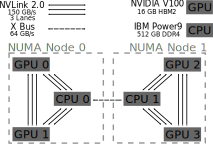
\includegraphics[width=0.8\textwidth]{figures/generated/hal-hardware.pdf}
    \label{fig:topo-ac922-simple}
\end{figure}

The IBM AC922 machine features two POWER9 CPUs and four Nvidia V100 GPUs~\cite{caldeira2018ac922}.
Each POWER9 CPU has 20 cores, with 4-way simultaneous multithreading, and is attached to 512GB of DDR4 memory for a total of 160 threads and 1TB of memory.
Each POWER9 CPU is part of a fully-connected triad of one POWER9 CPU and two V100 GPUs.
Each device in the triad is connected by three bonded NVLink 2.0 lanes for bidirectional bandwidth of 150 GB/s.
The two triads are connected at the POWER9 CPUs by an IBM SMP X bus with 64 GB/s bandwidth.
Table~\ref{tab:ac922} and Figure~\ref{fig:topo-ac922-simple} summarize the hardware configuration.
Like the S822LC, each triad is a Linux NUMA node.
